% vim: fdm=marker fmr=<<<,>>> fml=1 cole=0
% Preamble % <<<
% \documentclass[10pt,twocolumn,nobalancelastpage,aps,pra,superscriptaddress,nofootinbib,longbibliography%,linenumbers
% ]{revtex4-2}
\documentclass[fontsize=9pt,twoside=semi,bookmarkpackage=false]{scrartcl}

% \usepackage{libertinus}
\usepackage[a5paper,margin=10mm]{geometry}

% Have empty pages on new sections
% https://tex.stackexchange.com/a/85384/23298
% \usepackage{etoolbox}
% \pretocmd{\section}{\cleardoubleevenstandardpage}{}{}

\usepackage[mainfont]{ysabeau}
\renewcommand{\hbar}{\hslash}
\usepackage[small,euler-digits,euler-hat-accent]{eulervm}
\usepackage{xfrac}
\usepackage[mleftright]{diffcoeff}

\input{/home/omn/works/styles/latex/revtex4-1.tex}
\input{/home/omn/works/tmp/newcommands.tex}

\usetikzlibrary{external}
\tikzexternalize[prefix=tikz/]
\newcommand{\inputtikz}[1]{%
  \tikzsetnextfilename{#1}%
  \input{./tikz/#1.tikz}%
}

\usepackage{empheq}
\definecolor{mygr}{rgb}{0,0,.9}
\newcommand*{\mybx}[1]{\colorbox{mygr!15}{\hspace{1em}#1\hspace{1em}}}

\newcommand{\proptoinverse}{\mathrel{\mskip1mu\reflectbox{$\propto$}\mskip-1mu}}

\usepackage{appendix}

% \usepackage{autonum}

\usepackage{multicol}
\BeforeStartingTOC[toc]{\begin{multicols}{2}}
\AfterStartingTOC[toc]{\end{multicols}}

\begin{document}

% >>>

% TITLE <<<
  {
    \centering
    \textbf{\LARGE Exam Questions\\
      Quantum Statistical Optics
    }
    \\ \textcolor{gray}{\footnotesize version:\DTMNow }
    \par
  }

  \bigskip

% >>>

  {\footnotesize
  \tableofcontents
}

\section{Coherent, thermal and non-classical states of light, their properties and mathematical representation}% <<<

These states are quantum states of a harmonic oscillator (HO; see~\cref{sec:harmonic_oscillator} for more).

\subsection{Coherent states: Photon number distribution/ discrete variables (DV)} % <<<
\label{sec:photon_number_distribution}

Coherent states can be defined as eigenstates of the \emph{annihilation operator} $\hat a$ of the HO:
\begin{empheq}[box=\mybx]{equation}
  \label{eq:coh:ket:def}
  \hat a \ket{ \alpha } = \alpha \ket {\alpha },
\end{empheq}
where $\ket{\alpha}$ is the notation for the coherent state that uses a complex number $\alpha$.

We can write the coherent state in the basis of the energy levels of the HO (Fock states):
\begin{empheq}[box=\mybx]{equation}
  \ket{ \alpha } = \exp\left[- \frac{\abs{ \alpha }^2}{2} \right]
  \sum_{k=0}^\infty \frac{\alpha^k}{\sqrt{ k!}} \ket{k}.
\end{empheq}
The probability to obtain $m$ photons in a coherent state $\alpha$ then equals
\begin{empheq}[box=\mybx]{equation}
  p_m (\alpha) = \abs{ \braket{ m }{ \alpha }}^2
  = \ee^{ - \abs{ \alpha }^2 }
  \frac{ \abs{\alpha}^{2m} }{ m! }
  =
  \ee^{ - \ev{n} } \frac{ \ev{n }^m }{ m! },
\end{empheq}
where we denoted by $\ev{n}$ the mean number of phonons in this coherent state.
Example photon number distributions can be seen in~\cref{fig:probs_coh_therm}~(left).
It can be proven (we can compute it) that the mean number of photons and the variance of the photon number equal each other in the coherent state, because it follows Poisson distribution
\begin{align}
  \ev{n} & = \abs{ \alpha }^2,
  &
  \Var {n} & \equiv \ev{ n^2 } - \ev{ n }^2 = \ev{n } = \abs{ \alpha }^2.
\end{align}

\begin{figure}[htb]
  \centering
  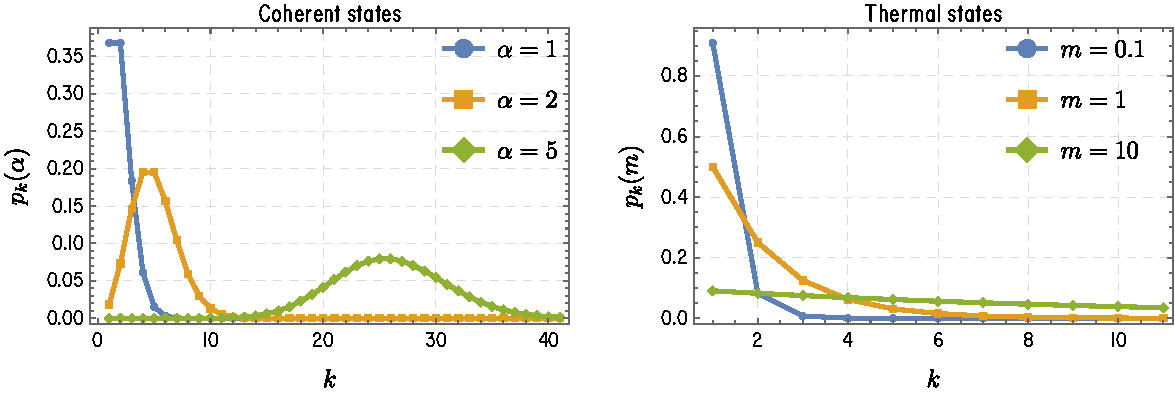
\includegraphics[width=0.99\linewidth]{probs_coh_therm}
  \caption{Probabilities to obtain $k$ photons in (left) coherent states and (right) thermal states for different parameters characterizing these states.}
  \label{fig:probs_coh_therm}
\end{figure}

We can also compute intensity autocorrelation function for a coherent state (pronounced "gee-two"):
\begin{equation}
  g^{(2)}_{\ket{ \alpha }}
  \equiv
  \frac{ \mel{\alpha}{ ( \hat a\dg )^2 \hat a ^2 }{\alpha} }{
  ( \mel{\alpha}{ \hat a\dg \hat a }{\alpha})^2 }
  = 1,
\end{equation}
when $\alpha \neq 0$.

% >>>
\subsection{Coherent states: Phase space properties/ continuous variables (CV)} % <<<
\label{sec:phase_space_properties}

Coherent states can be alternatively obtained as a result of application of the displacement operator $\hat D(\alpha)$ to the ground state $\ket {0}$ of the HO:
\begin{empheq}[box=\mybx]{align}
  \ket{\alpha } & = \hat D (\alpha ) \ket{ 0 },
  & \text{ where }
  \hat D (\alpha) & = \exp[ \alpha \hat a\dg - \alpha^* \hat a ].
\end{empheq}

This dictates that, similarly to the ground state, coherent states are Gaussian.
This means they have Gaussian wave functions, Wigner functions etc.
Gaussian states can be fully characterized by their first two statistical moments of quadratures.
These moments are the vector of mean values of the quadratures and the covariance matrix.

To compute these moments, we can use~\cref{eq:coh:ket:def} to compute expectations of the quadratures of the harmonic oscillator.
To perform computations, we reorder (if needed) the operators to have all $\hat a\dg$ to the left from all $\hat a$, then use the properties that
\begin{empheq}[box=\mybx]{align}
  \hat a \ket{\alpha} & = \alpha \ket{\alpha},
  & \text{ and }
  \bra{ \alpha } \hat a\dg & = \alpha ^* \bra{ \alpha }.
\end{empheq}
So
\begin{align}
  & \ev{ \hat q }_{\ket{\alpha}}
  = \mel{ \alpha }{ \hat q }{ \alpha }
  = \mel{\alpha}{ \hat a + \hat a\dg }{ \alpha }
  =
  \mel{\alpha}{ \hat a }{\alpha }
  + \mel{\alpha}{ \hat a \dg }{\alpha } = ( \alpha + \alpha ^* ) \braket{ \alpha }{ \alpha }
  = 2 \Re \alpha ,
  \\
  & \ev{ \hat p }_{ \ket{\alpha}}
  = \mel{ \alpha }{ \hat p }{ \alpha }
  = \mel{\alpha}{ ( \hat a - \hat a\dg )/ \ii }{ \alpha }
  = ( \alpha - \alpha ^* ) / \ii = 2 \Im \alpha .
\end{align}

For the second moments we can find
\begin{multline}
  \ev{ \hat q^2 }_{\ket{\alpha}}
  = \mel{ \alpha }{ \hat a^2 + (\hat a\dg)^2 + \hat a \hat a\dg + \hat a\dg \hat a }{ \alpha }
  = \mel{ \alpha }{ \hat a^2 + (\hat a\dg)^2 + 2 \hat a\dg \hat a + 1 }{ \alpha }
  \\
  = \alpha^2 + ( \alpha^* )^2 + 2 \alpha^* \alpha + 1
  = ( \alpha + \alpha^* )^2 + 1
  = ( 2 \Re \alpha )^2 + 1
  = \ev{ \hat q }_{\ket{ \alpha }}^2 + 1.
\end{multline}
Therefore, for the variance of the position quadrature we have
\begin{equation}
  \Var _{\ket{ \alpha }} \hat q  \equiv \ev{ \hat q^2 } - \ev{ \hat q }^2 = 1.
\end{equation}
We can show a similar result for $\hat p$, and that there are no cross-correlations between the quadratures.
As a result,
\begin{align}
  \Var q & = \Var p = 1,
  &
  \ev{ \hat q \hat p + \hat p \hat q } _{\ket{ \alpha }} = 0.
\end{align}
This is the same, as in the ground state of the HO $\ket{0}$.
This is quite expected, given that a coherent state is essentially a displaced ground state.

Therefore, the mean values of quadratures of a coherent state are defined by the coherent state label $\alpha$, and the second moments (variances) equal the ground state (shot-noise) variance.
We summarize this by writing the statistical moments of a coherent state $\ket{\alpha}$:
\begin{empheq}[box=\mybx]{align}
  \mvec \mu_\alpha & = 2 ( \Re \alpha , \Im \alpha )^\intercal,
  &
  \mmat V _\alpha & =
  \begin{pmatrix}
    1 & 0 \\ 0 & 1
  \end{pmatrix} = \mathbb{1}_2.
\end{empheq}

Note that the factor of $2$ in the mean values is the result of our choice of definitions of $\hat q, \hat p$:
\begin{align}
  \hat q & = \hat a + \hat a \dg
  &
  \hat p & = ( \hat a - \hat a\dg ) / \ii.
\end{align}
Consequently, $\comm{ \hat q }{ \hat p } = 2 \ii$.

Knowing the statistical moments of the quadratures, we can write the Gaussian Wigner function for coherent states.
Wigner function is a quasi-probability function that can take negative values for non-classical states.
Importantly, it is a real-valued function defined on the phase space, so it takes two real-valued arguments.
For a coherent state $\alpha$ it reads
\begin{empheq}[box=\mybx]{equation}
  W_{\ket{\alpha}} (q,p)
  =
  \frac{ 1 }{ 2 \pi }
  \exp\left[
  - \frac{ ( q - 2 \Re \alpha )^2 + ( p - 2 \Im \alpha)^2 }{ 2 }
  \right].
\end{empheq}

In particular, for the wave function in the position basis we can write
\begin{equation}
  \psi_{\alpha} (q) = \braket{ q }{ \alpha }
  =
  \frac{ 1 }{ \sqrt[4]{2 \pi }}
  \exp\left[ - \frac{ \left( x - 2 \Re(\alpha)\right)^2 }{ 4 } + \ii \Im \alpha x \right].
\end{equation}

Lastly, different coherent states are not orthogonal
\begin{equation}
  \braket{ \beta }{ \alpha }
  = \exp\left[- \frac 12 (|\beta|^2+|\alpha|^2-2\beta^*\alpha)\right]\neq\delta(\alpha-\beta).
\end{equation}
For orthogonal states, we'd have $\braket{ \alpha }{ \beta } = 0$ as long as $\alpha \neq \beta$.

% >>>
\subsection{Non-classical states} % <<<
\label{sec:nonclassical_states}

Coherent states form an overcomplete basis, in which other quantum states can be expanded.
So, for an arbitrary state $\rho$, one can write its expansion over coherent states:
\begin{empheq}[box=\mybx]{align}
  \hat \rho = \int \dl{ \Re \alpha} \dl{ \Im \alpha} \: P_\rho (\alpha) \projector{\alpha}.
\end{empheq}
This is called the \emph{Glauber-Sudarshan} representation, and $P_\rho$ is called \emph{the $P$-function} or \emph{Glauber-Sudarshan $P$-function}.
This representation is used to distinguish classical states from non-classical.
Those states for which their $P$-function is a regular probability distribution, are said to be classical.
Other states are non-classical.

The definition above tells that classical statistical mixtures of coherent states are also classical.
Statistical mixtures of coherent states cannot have variances of quadratures lower than the variance of the coherent state (shot noise).
Correspondingly, a quantum state that shows squeezing in any quadrature, is necessarily non-classical.

% >>>
\subsection{Thermal states} % <<<
\label{sec:thermal_states}

Thermal states $\hat \rho\s{th}(m)$ are classical mixed states of a HO.
They are characterized by a single real number $m > 0$ which is the mean occupation (mean number of photons):
\begin{equation}
  \ev{ \hat n } = \ev{ \hat a\dg \hat a } = \Tr( \hat \rho\s{th} (m) \hat a\dg \hat a ) = m.
\end{equation}

For a physical oscillator of the frequency $\omega$ in thermal equilibrium with the environment at temperature $T$, the mean number of photons (or phonons) is defined by the Bose-Einstein statistics:
\begin{equation}
  m = \left( \exp\left[ \hbar \omega / ( k\s{B} T )\right] - 1 \right)^{-1}
  \approx \frac{ k\s{B} T }{ \hbar \omega },
\end{equation}
where $\hbar$ is the reduced Planck's constant, $k\s{B}$ is Boltzmann's constant.
For light frequencies even at room temperature $m = 0$ to a good accuracy.
Thermal state with $m=0$ is the ground state.

In the Fock basis, thermal state can be written as
\begin{empheq}[box=\mybx]{align}
  \hat \rho\s{th} (m) & = \sum_{k = 0 }^\infty p\s{th} (k; m) \projector{k},
  &
  \text{ where }
  p\s{th} ( k; m) & = \frac{ m^k }{ ( 1  + m )^{k + 1 } }.
\end{empheq}
Example photon number distributions can be seen in~\cref{fig:probs_coh_therm}~(right).

The intensity autocorrelation for a thermal state equals two:
\begin{equation}
  g^{(2)}\s{th} = 2,
\end{equation}
when $m \neq 0$.

Thermal state is Gaussian, with zero mean values of both quadratures and symmetric covariances:
\begin{empheq}[box=\mybx]{align}
  \mvec \mu\s{th} & = 0,
  &
  \mmat V\s{th} (m) & =
  \begin{pmatrix}
    2 m + 1 & 0 \\ 0 & 2 m + 1
  \end{pmatrix}
  = ( 2 m + 1 ) \mathbb{ 1 }.
\end{empheq}
We can write the Wigner function of this Gaussian state:
\begin{empheq}[box=\mybx]{align}
  W\s{th} (q ,p; m ) =
  \frac{ 1 }{ 2 \pi ( 2 m + 1 ) }
  \exp\left[ - \frac{ 1 }{ 2 }\cdot \frac{ q^2 + p^2 }{ 2 m + 1 } \right].
\end{empheq}

\begin{figure}[htb]
  \centering
  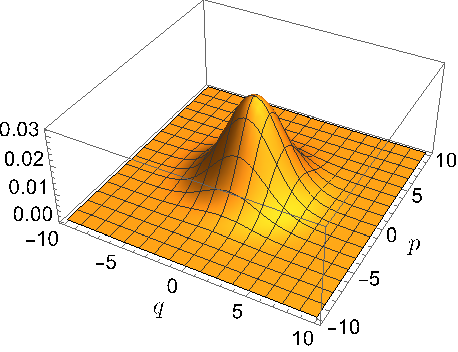
\includegraphics[width=.49 \linewidth]{therm3d.pdf}
  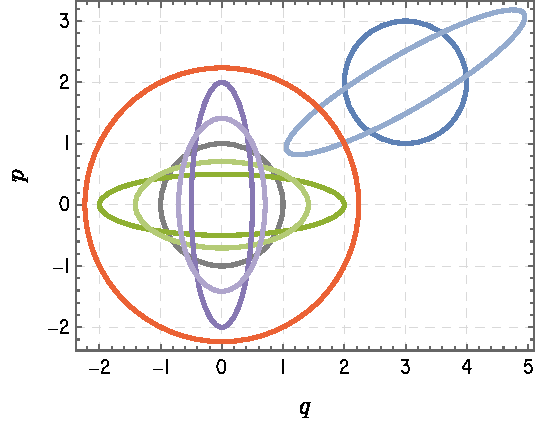
\includegraphics[width=.49 \linewidth]{ellipses.pdf}
  \caption{Illustrations of Gaussian quantum states.
    Left: a thermal state with $m = 2$ photons.
    Right: ellipses showing variances of different states.
    The ellipses are centered at mean values of quadratures corresponding to these states.
  Gray: ground state $\ket{0}$, red: thermal state with $m = 2$ photons; green, purple: squeezed states (green: squeezed in momentum; purple: squeezed in position); dark blue: coherent state with $2 \alpha = 3 + 2 \ii$; light blue: displaced squeezed state. }
  \label{fig:gaussian_plots}
\end{figure}

% >>>
\subsection{Squeezed states} % <<<
\label{sec:squeezed_states}

Applying a squeeze operator $\hat S (\zeta) = \exp\left[ \frac 12 ( \zeta^* \hat a^2 -  \zeta ( \hat a\dg )^2 )\right]$ to the ground state $\ket{0}$ of a HO, one can obtain \emph{squeezed states}:
\begin{equation}
  \ket{ \zeta } = \hat S (\zeta) \ket{0}.
\end{equation}
The parameter $\zeta = r \ee^{ \ii \phi }$ is called the squeezing parameter and can be complex.
Often it is separated into the real-valued squeezing magnitude $r$ and the real-valued squeezing phase $\phi$.

With $r\neq 0$, the resulting squeezed states are non-classical Gaussian quantum states.
They have zero mean values of the quadratures, and the covariance matrix describing an ellipse in the phase space.
In particular, for $\phi = 0$,
\begin{align}
  \label{eq:squeez.st}
  \mvec \mu\s{S} & = \mvec 0, &
  \mmat V\s{S} & =
  \begin{pmatrix}
    \ee^{ - 2 r } & 0 \\
    0 & \ee^{ 2 r }
  \end{pmatrix}.
\end{align}
That is, the variance of the position is suppressed, the variance of momentum is enlarged.
Importantly, the determinant of the covariance matrix remains fixed.
For different values of $\phi$, squeezed will be a different quadrature, however an orthogonal quadrature will always be anti-squeezed.

The Wigner function for the state with statistics given by~\cref{eq:squeez.st} reads
\begin{equation}
  W_S ( q , p ) = \frac{ 1 }{ 2 \pi }
  \exp \left[ - \frac 12
  \left( x^2 \ee^{ 2 r } + p^2 \ee^{ -2 r } \right) \right].
\end{equation}

Since squeezed states have variances of some quadratures suppressed below the shot-noise level, these states are non-classical.
It is easy to show that when we take a statistical mixture of two or more coherent states, the variance of any quadrature cannot be made smaller than the variance corresponding to the ground state.

% >>>
\subsection{Displaced squeezed and squeezed coherent states} % <<<
\label{sec:displaced_squeezed_states}

Combination of displacement and squeezing can produce non-classical states.

First, displacing a squeezed state does not change its covariance matrix, therefore, a squeezed state, initially non-classical, preserves its non-classicality upon displacement.
Second, squeezing a coherent state will squeeze variance of some quadrature, and make the resulting state non-classical.

Importantly, the operations of squeezing and displacement, do not commute, that is their order matters:
\begin{equation}
  \hat S ( \zeta ) \hat D ( \alpha )  \neq \hat D (\alpha ) \hat S ( \zeta ).
\end{equation}
On the other hand, one can always find another pair of squeezing and displacement parameters $(\alpha', \zeta')$ such that
\begin{equation}
  \hat S ( \zeta ) \hat D ( \alpha ) = \hat D (\alpha' ) \hat S ( \zeta' ).
\end{equation}

Either way, the Gaussian parameters of the resulting states will have a non-zero vector of mean values of the quadratures and a covariance matrix corresponding to a squeezed state, e.g.:
\begin{align}
  \mvec \mu\s{DS} & =
  \begin{pmatrix}
    \ev{q} \\ \ev{ p}
  \end{pmatrix},
  &
  \mmat V\s{DS} & =
  \begin{pmatrix}
    \ee^{ - 2 r } & 0
    \\
    0 & \ee^{ 2 r }
  \end{pmatrix}.
\end{align}

% >>>
\subsection{Fock states} % <<<
\label{sec:fock_states}

As we know, classical are the coherent states and their classical mixtures (equivalently, incoherent statistical mixtures).
All the remaining states are non-classical.
Text-book examples of non-classical states are the Fock states.

Fock states $\ket{k}$ with $k = 0,1,2,\dots$ are the energy levels of harmonic oscillator.
These states form an orthonormal basis (each state is normalized, and they are orthogonal to each other):
\begin{equation}
  \braket{ m }{ n } = \delta_{mn },
\end{equation}
where $\delta$ is the Kronecker delta-symbol.
Any pure state $\ket \psi$ can be expanded over the basis of the Fock states:
\begin{equation}
  \ket{ \psi } = \sum_{n = 0}^\infty \braket{ n }{ \psi } \ket{n }
  \equiv \sum_{n = 0}^\infty C_n \ket{ n }.
\end{equation}

The probability to obtain $n$ photons having a state $\ket{k}$ is quite straightforwardly,
\begin{equation}
  p_n (k) = \delta_{nk },
\end{equation}
The probability is $1$ when $n = k$ and zero otherwise.

The intensity autocorrelation for the Fock states reads
\begin{empheq}[box=\mybx]{equation}
  \label{eq:g2fock}
  g^{(2)}_{\ket{k}}
  = \frac{ \mel{ k }{ ( a \dg )^2 a^2 }{ k } }{ \mel{ k }{ a\dg a }{ k }^2 }
  = \frac{ k ( k - 1 ) }{ k^2 } = 1 - \frac 1 k,
\end{empheq}
when $k \neq 0$.

The intensity autocorrelation shows the probability of simultaneous detection of multiple photons.
\cref{eq:g2fock} shows that for the Fock states it is suppressed.
In particular, for $k = 1$, $g^{(2)}_{\ket 1} = 0$, so the probability of detection of multiple photons is zero.
The corresponding effect is called \emph{anti-bunching} of photons.

The wave-function of a Fock state in the position basis is (up to normalization)
\begin{equation}
  \psi_n (q) = \braket{ q }{ n }
  \propto H_n \left( \frac{ q }{ \sqrt{ 2 }} \right)
  \exp\left[ - \frac{ q ^2 }{ 4 } \right],
\end{equation}
where $H_n$ are Hermite polynomials.

In quantum optics, the Wigner function is used often:
\begin{empheq}[box=\mybx]{equation}
  W_n (q , p ) = \frac{ ( -1 )^{-1} }{ 2 \pi }
  \exp\left[ - \frac{ q^2 + p^2 }{ 2 } \right]
  L_n ( q^2 + p^2 ).
\end{empheq}
Here $L_n$ are Laguerre polynomials.
In particular,
\begin{align}
  L_0 (x) & = 1, &
  L_1 (x) & = 1 - x, &
  L_2 (x) & = 1 - 2 x + x^2 / 2.
\end{align}
Obviously, these Wigner functions are rotationally symmetric (don't change under rotation of the phase space).

Wigner functions of Fock states are illustrated in~\cref{fig:plt_wig_fock}.

\begin{figure}[htb]
  \centering
  % 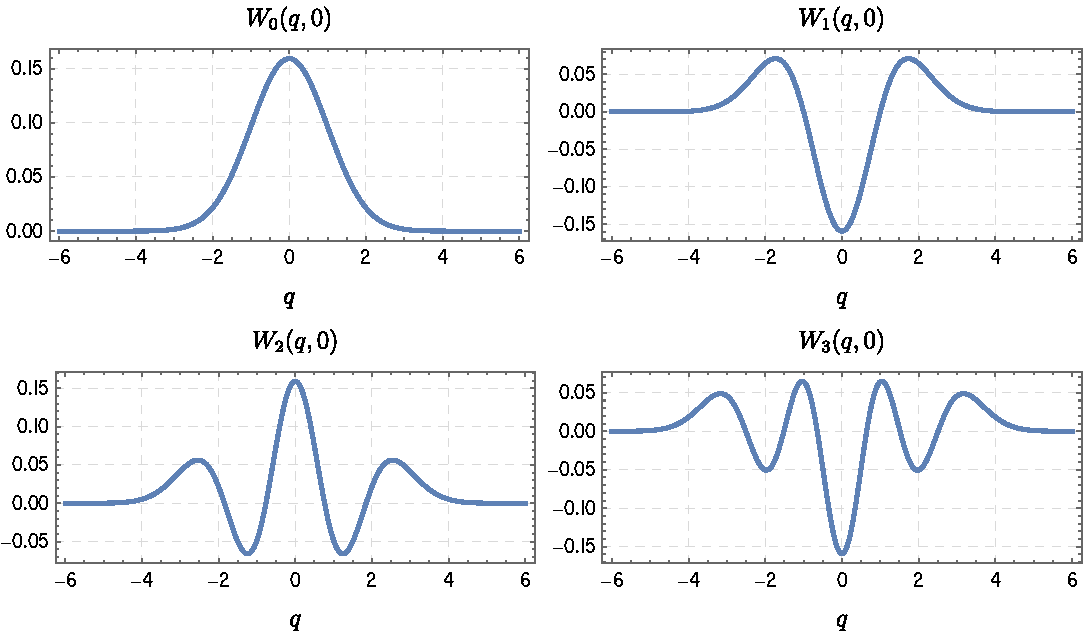
\includegraphics[width=0.58\linewidth]{plt_wig_indiv}
  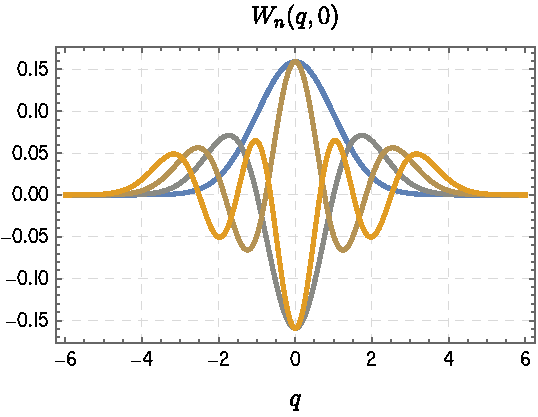
\includegraphics[width=0.5\linewidth]{plt_wig_grp}
  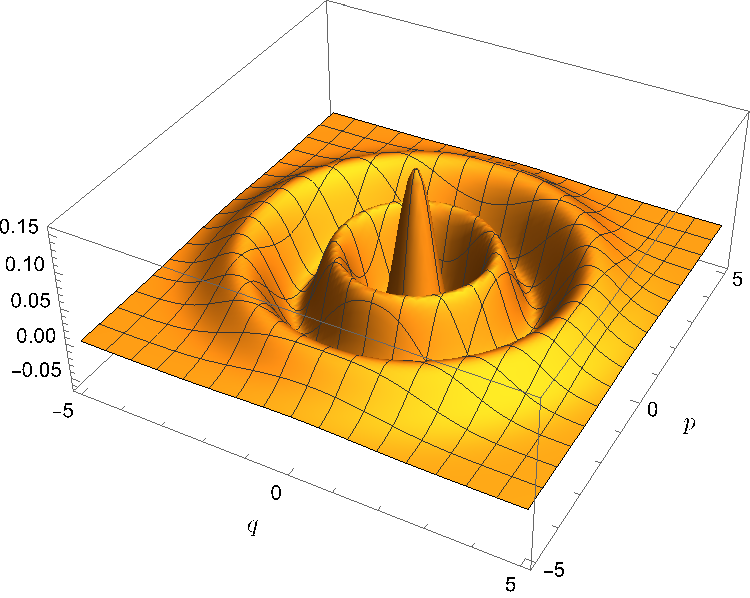
\includegraphics[width=0.4\linewidth]{plt_wig3d}
  \caption{
    Left: cuts of Wigner functions of the Fock states $\ket{0}$ to $\ket{3}$.
    Right: Wigner function $W_4(q,p)$ of the Fock state $\ket{4}$.
  }
  \label{fig:plt_wig_fock}
\end{figure}

% >>>
\subsection{Other non-classical states} % <<<
\label{sec:other_non_classical_states}

There are many more non-classical states then described previously.
Though it can be challenging to create non-classical states experimentally.
Different strategies to create non-classical states include adding and subtracting photons or using nonlinearities.

% >>>

% >>>

\cleardoublepage

\section{Isolated and open quantum dynamics of quantum states of light and atoms, description and basic models} % <<<
\label{sec:isolated_and_open_quantum_dynamics_of_quantum_states_of_light_and_atoms_description_and_basic_models}

We start with a description of the dynamics of isolated systems, then outline some approaches to open systems.

\subsection{Isolated quantum systems} % <<<
\label{sec:isolated_quantum_systems}

Normally, dynamics of the isolated quantum system can be described by its \emph{Hamiltonian} (operator of energy) $\hat H$.
The ``dynamics'' means evolution of the quantum state.
The quantum state of a quantum system at each time is described by the state vector (equivalently, wave-function) $\ket{ \psi (t) }$.
The evolution of the state vector is given by the Schrödinger equation
\begin{empheq}[box=\mybx]{equation}
  \diff{}{ t }  \ket{ \psi(t) }= \frac{ 1 }{ \ii \hbar } \hat H \ket{ \psi (t) }.
\end{empheq}
Its solution can be written as
\begin{empheq}[box=\mybx]{equation}
  \label{eq:closed:shrodingerpic}
  \ket{ \psi (t) } = \hat U (t , t_0) \ket{ \psi (0) },
\end{empheq}
where $\hat U (t,t_0)$ is a \emph{unitary} operator (meaning $\hat U \hat U\dg = \hat 1$) that equals
\begin{empheq}[box=\mybx]{equation}
  U (t,t_0) = \exp\left[ - \ii \hat H ( t - t_0) / \hbar \right].
\end{empheq}

When we have an observable $\hat A$ and want to compute its statistics (say, mean value) as a function of time, we have to substitute $\ket{ \psi (t)}$.
Then we have
\begin{equation}
  \ev{ \hat A } _{\ket{ \psi }} (t)
  = \mel{ \psi (t) }{ \hat A }{ \psi (t) }
  = \mel{ \psi (t_0) }{ \hat U\dg (t, t_0) \hat A \hat U (t , t_0) }{ \psi (0) }
  = \mel{ \psi (0) }{ \hat A\s{H} (t) }{ \psi (0) },
\end{equation}
where $\hat A\s{H}(t)$ defined as
\begin{empheq}[box=\mybx]{equation}
  \hat A\s{H} (t) = \hat U\dg (t , t_0) \hat A \hat U (t, t_0)
\end{empheq}
is the operator in the \emph{Heisenberg picture}.
At the initial time $t = t_0$, the operators in Heisenberg picture and Schrödinger picture coincide: $\hat A\s{H} (t_0) = \hat A$.

We can show that the operator in the Heisenberg picture satisfies the Heisenberg equation
\begin{empheq}[box=\mybx]{equation}
  \label{eq:heisenberg:eqn}
  \diff{ \hat A\s{H} (t) }{ t } = \frac{ \ii }{ \hbar } \comm{ \hat H }{ \hat A\s{H} }
  = \frac{ \ii }{ \hbar } \comm{ \hat H }{ \hat A }.
\end{empheq}

Lastly, we have to consider the case when our isolated system is initially in a mixed (not pure) state.
Then it does not have the state vector $\ket{ \psi }$ but rather is described by the density matrix $\hat \rho$.
In Schrödinger picture, the density matrix obeys \emph{von Neumann} equation
\begin{empheq}[box=\mybx]{equation}
  \label{eq:vonneumann:eqn}
  \diff{}{t} \hat \rho (t) = \frac{ \ii }{ \hbar } \comm{ \hat \rho }{ \hat H }.
\end{empheq}
Its solution reads
\begin{equation}
  \rho (t) = \hat U (t, t_0 ) \hat \rho (t_0) \hat U \dg (t, t_0).
\end{equation}
Note the different order of the operators $\hat U$ and $\hat U\dg$ in the solutions for $\hat A\s{H} (t)$ and $hat \rho (t)$.
Also, different order of operators in the commutators in~\cref{eq:heisenberg:eqn,eq:vonneumann:eqn}.

Summary: we will mostly use~\cref{eq:heisenberg:eqn,eq:vonneumann:eqn}.

% >>>
\subsection{Atom-light interaction: formulation} % <<<
\label{sec:atom_light_interaction}

Atom-light interaction is a very broad topic.
The standard textbook by Scully \& Zubairy uses about 80 pages for the two chapters dedicated to atom-light interaction.

\begin{figure}[htb]% <<<
  \centering
  \inputtikz{atom-cavity}
  \caption{Atom-light interaction illustration.
    On the left, an atom is placed inside an optical cavity formed by the two mirrors.
    In the middle, the energy level diagram of the atom.
  On the right, the energy level diagram of the field in the cavity.}
  \label{fig:atom:light:int}
\end{figure}% >>>

The key models to study here are the Rabi model and the Jaynes-Cummings model.
Both the models consider interaction of a two-level atom with light inside an optical cavity.
The Hamiltonian for such a system reads
\begin{equation}
  \hat H = \hat H\s{A} + \hat H\s{cav} + \hat H\s{int},
\end{equation}
where $\hat H\s{A}$ is the Hamiltonian of a bare atom,
$\hat H\s{cav}$ is the Hamiltonian of the bare cavity, and $\hat H\s{int}$ is the interaction Hamiltonian.

In more detail, the optical cavity is a harmonic oscillator of frequency $\omega\s{c}$ with the annihilation operator $\hat a$, so
\begin{equation}
  \hat H\s{cav} = \hbar \omega\s{cav} \hat a\dg \hat a.
\end{equation}

The ``two-level atom'' is an atom such that only two its energy sublevels can be addressed by the light.
The other levels do not take part in the interaction, so the atom effectively has only two energy levels.
The two levels are normally denoted $\ket{g}$ (for the lower level) and $\ket{e}$ (for the higher energy level), with energies $E_e > E_g$.
The values of these energies are insignificant on their own, but what matters is the energy difference:
\begin{equation}
  \frac{ E_e - E_g }{ \hbar } = \omega_q.
\end{equation}
This is the transition frequency of the atom, and this is the only number that fully describes the atom.
The Hamiltonian of the atom reads
\begin{equation}
  \hat H\s{A}
  = \frac{ \hbar \omega_q }{ 2 } \sigma_z
  = \frac{ \hbar \omega_q }{ 2 }
  \begin{pmatrix}
    1 & 0 \\ 0 & - 1
  \end{pmatrix}.
\end{equation}
Here $\sigma_z$ is a Pauli matrix.
Note that we write the matrix of the Hamiltonian operator.
We do this in the basis of the energy levels of the atom, so we can expand it to the full form as
\begin{equation}
  \hat H\s{A}
  = \frac{ \hbar \omega_q }{ 2 }
  \bigg[ \projector{e} -  \projector{g} \bigg].
\end{equation}

Finally, the interaction between cavity light and the atom is assumed to be a dipole interaction.
From classical electrodynamics, the interaction between a dipole moment $\mvec d$ and the electric field $\mvec E$ equals $\mathcal H = - \mvec d \cdot \mvec E$.
Now we represent the dipole moment in terms of the atom operators:
\begin{equation}
  \hat { \mvec d } = \hat \sigma_+ d + \hat \sigma_- d^*,
\end{equation}
where $d$ is a dimensional coefficient, and
\begin{align}
  \sigma_+ & =
  \begin{pmatrix}
    0 & 1 \\ 0 & 0
  \end{pmatrix},
  &
  \sigma_- = \sigma_+\dg & =
  \begin{pmatrix}
    0 & 0 \\ 1 & 0
  \end{pmatrix}.
\end{align}
Then, we represent the electric field $\mvec E$ as
\begin{equation}
  \hat{\mvec E }= A \hat a + A^* \hat a\dg,
\end{equation}
where $A$ is a dimensional coefficient.

Collecting everything together, the interaction Hamiltonian reads
\begin{equation}
  \hat H\s{int} = \hbar g (\hat \sigma_+ +\hat \sigma_- ) ( \hat a + \hat a\dg ),
\end{equation}
where we for simplicity assumed $d = d^*$ and $A = A^*$, and introduced the coupling rate $g = A d / \hbar$.
Moreover, strictly speaking, above $d$ has to be a vector including geometric properties of the atom, and $A$ also has to be a vector taking into account polarization of light.
The scalar product of these two quantities will contribute to the coupling rate $g$.

Collecting together the parts of the atom-light Hamiltonian, we can finally write the full Hamiltonian:
\begin{empheq}[box=\mybx]{equation}
  \hat H\s{A-L} =
  \hbar \omega\s{cav} \hat a \dg \hat a
  + \frac 12 \hbar \omega_q \hat \sigma_z
  + \hbar g (\hat \sigma_+ +\hat \sigma_- ) ( \hat a + \hat a\dg ).
\end{empheq}
This Hamiltonian will be the starting point for the subsequent discussion.

% >>>
\subsection{Atom-light interaction: Rabi model} % <<<
\label{sec:atom_light_interaction_rabi_model}

The Rabi model assumes the light to be a classical field following a harmonic law:
\begin{equation}
  ( \hat a + \hat a\dg ) = E(t) = \varepsilon \cos ( \omega\s{cav} t  ).
\end{equation}
The first term (the light Hamiltonian) can be discarded: if the field is classical, this first term will become simply a complex number.
In all quantum pictures it will commute with every operator and will thus not contribute to the equations of motion.

% >>>
\subsection{Open quantum systems: General notes} % <<<
\label{sec:open_quantum_systems}

The usual approach to open quantum systems is as follows (see~\cref{fig:opensys}).
The system in consideration is extended to include not only the studied system itself (``System''), but also its environment (``Bath'') with which the system interacts in an attempt to get the solution for the compound system.
Normally some assumptions are made about the environment and the type of the system-bath interaction to simplify the solutions.
Afterwards, the environment is traced out to obtain the effective equations for the system of interest.
This tracing out can involve e.g. taking the average over the bath variables or something similar, and depends on the approach.

The two common approaches to open systems are
\begin{itemize}
  \tightlist
  \item Heisenberg-Langevin equations of motion
  \item master equations (Lindblad, Bloch-Redfield, \dots)
\end{itemize}

\begin{figure}[htb]
  \centering
  \inputtikz{open_systems}
  \caption{Illustration of an open system being embedded into a larger system (environment).}
  \label{fig:opensys}
\end{figure}

% >>>

% >>>

\cleardoublepage

\appendix
\appendixpage
\addappheadtotoc

\section{Harmonic oscillator} % <<<
\label{sec:harmonic_oscillator}

Harmonic oscillator (HO) is a system with the Hamiltonian that equals
\begin{equation}
  \hat H\s{HO} = \hbar \omega ( \hat a\dg \hat a +  \sfrac 12 ) \equiv \hbar \omega ( \hat n + \sfrac 12 ),
\end{equation}
where $\omega$ is the frequency of the oscillator, $\hat a$ is the \emph{annihilation} operator, $\hat a\dg$ is the \emph{creation} operator, $\hat n$ is the \emph{photon-number} operator.
The operators $\hat a, \hat a\dg$ are sometimes called the \emph{ladder} operators or \emph{bosonic} operators.
These operators satisfy the \emph{fundamental/canonical commutation relation}
\begin{equation}
  \comm{ \hat a }{ \hat a \dg } = 1.
\end{equation}

Energy levels of the HO are called \emph{Fock} states:
\begin{equation}
  \hat H\s{HO} \ket{ k } = E_k \ket{ k } = \hbar \omega ( k + \sfrac 12 ) \ket{ k },
  \qquad
  \text{ for }
  k = 0,1,2,\dots
\end{equation}

Operators $\hat a, \hat a\dg$ perform jumps between the levels:
\begin{align}
  \hat a \ket{ k }        & = \sqrt{ k } \ket{ k - 1 }, &
  \hat a\dg \ket{ k - 1 } & = \sqrt{ k } \ket {k }.
\end{align}
Note that $\hat a \ket{0} = 0$.

It is convenient to introduce the \emph{quadrature} operators:
\begin{align}
  \hat q & = \hat a + \hat a\dg, &
  \hat p & = ( \hat a - \hat a\dg ) / \ii.
\end{align}
These operators satisfy the following canonical commutation relation: $\comm{ \hat q }{ \hat p } = 2 \ii$.

It is convenient to describe HO with their Wigner function.
For a Gaussian state with the vector of means $\mvec \mu$ and covariance matrix $\mmat V$, the Wigner function reads
\begin{equation}
  W_G ( q , p ; \mvec \mu, \mmat V )
  =
  \frac{ 1 }{ 2 \pi \sqrt{ \det \mmat V }}
  \exp\left[
    - \frac 12 \mvec d^\intercal \mmat V^{-1}  \mvec d
  \right],
\end{equation}
where $\mvec d$ is the vector of deviations from the mean values:
\begin{equation}
  \mvec d
  =
  \begin{pmatrix}
    q - \ev{ \hat q } \\ p - \ev{ \hat p }
  \end{pmatrix}
  =
  \begin{pmatrix}
    q \\ p
  \end{pmatrix}- \mvec \mu.
\end{equation}

% >>>
\section{Two-level system} % <<<
\label{sec:two_level_system}

Two-level system, equivalently, a qubit, is a quantum system that has two basis states or energy levels.
Normally, they are denoted $\ket{e}$ and $\ket{g}$ or $\ket{\uparrow}$ and $\ket{\downarrow}$.
The associated energies are $E_e$ and $E_g$.
The Hamiltonian reads in the basis of energy levels:
\begin{equation}
  \hat H = E_e \projector{e} + E_g \projector{g}
  \equiv
  E_e
  \begin{pmatrix}
    1 & 0 \\ 0 & 0
  \end{pmatrix}
  +
  E_g
  \begin{pmatrix}
    0 & 0 \\ 0 & 1
  \end{pmatrix}
  =
  \begin{pmatrix}
    E_e & 0 \\ 0 & E_g
  \end{pmatrix}
  ,
\end{equation}
where we just wrote explicitly the projector operators in the matrix form.
Energy levels are eigenstates of the Hamiltonian, so in the basis of its eigenstates, the operator is diagonal.
The entries on the main diagonal in this basis are the eigenvalues.

We can rewrite the Hamiltonian as
\begin{multline}
  \label{eq:qubit:hamiltonian}
  \hat H =
  \begin{pmatrix}
    E_e & 0 \\ 0 & E_g
  \end{pmatrix}
  =
  \begin{pmatrix}
    \frac 12 \left[ E_e - E_g \right] + \frac 12 \left[ E_e + E_g \right]a & 0
    \\
    0 &
    \frac 12  \left[ E_g - E_e \right] + \frac 12 \left[ E_g + E_e \right]
  \end{pmatrix}
  \\
  =
  \frac 12 ( E_e - E_g )
  \begin{pmatrix}
    1 & 0 \\ 0 & -1
  \end{pmatrix}
  + \frac 12 ( E_e + E_g )
  \begin{pmatrix}
    1 & 0 \\ 0 & 1
  \end{pmatrix}
  =
  \frac 12 ( E_e - E_g ) \sigma_z + \frac 12 ( E_e + E_g ) \mathbb 1.
\end{multline}
Where we used e.g.
\begin{equation}
  E_e = \frac 12 E_e + \frac 12 E_e + \frac 12 E_g - \frac 12 E_g
  =
  \frac 12 ( E_e - E_g ) + \frac 12 ( E_e + E_g ).
\end{equation}

Note that in~\cref{eq:qubit:hamiltonian} the last term is proportional to the identity operator.
The identity commutes with everything, therefore, it will have no effect on any equations of motion and consequently, no effect on the quantum dynamics at all.
Therefore, we can safely ignore it.
The only remaining term is proportional to $\sigma_z$:
\begin{equation}
  \hat H = \frac 12 ( E_e - E_g ) \sigma_z = \frac 12 \hbar \omega_q \sigma_z,
\end{equation}
where we define  the transition frequency between the two levels as $\omega_q = ( E_e - E_g ) / \hbar$.

% >>>

% \bibliography{/home/omn/works/refs}
\end{document}
